%%
%% CSD Assignment 1 - Final Technical Report
%% AI-based Village Pond Planning System
%%
\documentclass[manuscript,screen,review]{acmart}

\AtBeginDocument{%
  \providecommand\BibTeX{{Bib\TeX}}}

\usepackage{tikz}
\usetikzlibrary{arrows.meta}

% \setcopyright{acmlicensed}
% \acmConference[CSD Assignment 1]{Course: Computer Science and Design}{2026}{Your Institute}
% \acmISBN{}

\begin{document}

%% =================== TITLE & AUTHOR BLOCK =========================
\title{AI-based Village Pond Planning System}
\subtitle{CSD Assignment 1 -- Final Technical Report}

\author{Akshat Gupta}
\affiliation{%
  \institution{Indian Institute of Technology Bhilai, Dept. of Data Science and Artificial Intelligence (Roll No. 12340160)}
  \country{India}}
\email{akshatg@iitbhilai.ac.in}

\renewcommand{\shortauthors}{Gupta}

%% =================== ABSTRACT ======================================
\begin{abstract}
Rural India depends on small ponds to store monsoon rainfall for the dry months, but
choosing where to dig one is usually still done by eye. A good site needs a catchment
large enough to fill the pond, ground that drains but is flat enough to build on, and
safe distance from the nearest stream. This report presents a web application that
automates that choice. A user draws an area on a map, or uploads a surveyed contour
sheet, and the system returns a recommended pond location, its catchment area, and its
expected annual water yield, all drawn on the map. Elevation comes from free SRTM
satellite tiles or from the uploaded survey. Ten years of daily rainfall come from the
Open-Meteo archive. The catchment is traced by routing water downhill across the
elevation grid with D8 flow routing, and runoff is estimated day by day with the SCS
curve number method rather than as one annual storm. The system was checked by running
the same ground through both data paths: the free elevation tiles reproduce a provided
1 m survey to 0.26 m RMSE, and the two paths recommend a pond site 402 m apart in the
same valley. Under load on four containers capped at 512 MB each, matching the
deployment limit for this assignment, the system answers a village-scale query in
about half a second and holds a peak memory of 276 MiB. 588 automated tests cover the
terrain analysis, the API, and the agreement between the two data paths.
\end{abstract}

\keywords{Village Pond Planning, Geospatial Analysis, Rainwater
  Harvesting, Catchment Estimation, Web GIS, REST APIs}

\maketitle

\begingroup\footnotesize\noindent
\textbf{Project links.} Code: \url{https://github.com/Akshats-git/Pond-Catchment-Analysis} ~~
Live app: \url{http://10.1.75.53:5229/} ~~
Video: \url{https://youtu.be/r1ir7I915W4}
\endgroup
\par\smallskip

%% =====================================================================
\section{Introduction}
\label{sec:intro}

Villages across central India rely on small ponds to catch monsoon rain and carry a
household or a few fields through the dry season. Building a pond in the wrong place
wastes both money and water. Too small a catchment and it never fills. Too close to a
stream and the first flood destroys it. Deciding where to build has traditionally been
left to local judgement, because the elevation data, rainfall records and land maps
needed to do it properly are scattered across different offices and rarely combined.

This project builds a web application that makes that decision faster and more
consistent. A user marks a piece of land on a map, or uploads a surveyed contour sheet
if one exists, and the system works out where a pond should go, how much land drains
into it, and how much water it can expect to collect in an average year. All of this is
drawn back onto the same map.

The rest of this report is organised as follows. Section~\ref{sec:requirements} restates
the assignment's requirements. Section~\ref{sec:architecture} describes the system
architecture. Section~\ref{sec:methodology} explains the terrain and hydrology
methodology. Section~\ref{sec:implementation} covers the implementation.
Section~\ref{sec:csd-themes} maps the project onto core computer system design themes.
Section~\ref{sec:results} presents results and measured performance.
Section~\ref{sec:discussion} discusses limitations, and Section~\ref{sec:ai-usage}
declares how AI tools were used.

\subsection{Motivation}
Manual site selection is hard for three reasons. First, the terrain itself is not
simple. Water does not flow downhill in a straight line, it collects along specific
channels that are not obvious from a satellite photo alone. Second, rainfall records
are not centralised, so a village-level annual figure usually has to be estimated from
a distant weather station or a published climatology. Third, land records that show
what ground is already built on, already under water, or otherwise unavailable are not
in a form a village administrator can search. An automated tool that reads elevation
and rainfall from free data sources removes all three obstacles at once and gives a
quantified answer, a catchment area in hectares and a volume in cubic metres, instead
of a guess.

\subsection{Scope of the Project}
The system, given a chosen area or an uploaded contour sheet, does the following:
estimates a digital elevation model, recommends a pond site and up to four
alternatives, estimates catchment area with an uncertainty band, estimates annual
water yield from historical rainfall, generates a stage-storage curve and a pond
capacity for a chosen depth, overlays all of this on an interactive map, flags
existing ponds and unavailable land from satellite imagery, and lets a user save and
export the result.

It does not perform structural or civil engineering design of the pond embankment. It
does not verify land ownership or the legal availability of the chosen site. It does
not guarantee construction-grade accuracy from data at 17.8 m to 30 m resolution; a
formal survey is still recommended before building. It does not analyse drinking-water
quality.

%% =====================================================================
\section{Problem Statement and Requirements}
\label{sec:requirements}

Table~\ref{tab:requirements} maps the assignment's stated functional requirements onto
the module that satisfies each one.

\begin{table}[h]
  \caption{Functional requirements and where they are implemented}
  \label{tab:requirements}
  \begin{tabular}{p{3.6cm}p{3.6cm}}
    \toprule
    Requirement & Implemented in \\
    \midrule
    Satellite imagery display & Esri imagery basemap, \texttt{static/index.html} \\
    Contour map visualization & \texttt{app/core/contouring.py} and the map overlay \\
    Available-land identification & \texttt{app/cv/imagery.py}, \texttt{/land/available} \\
    Catchment area estimation & \texttt{app/core/catchment.py} \\
    Historical rainfall query & \texttt{app/providers/rainfall.py}, \texttt{/rainfall} \\
    Runoff volume estimation & \texttt{app/core/hydrology.py} \\
    Pond depth / storage recommendation & \texttt{app/core/hydrology.py}, stage-storage curve \\
    Combined overlay / results view & \texttt{static/index.html} results panel \\
    \bottomrule
  \end{tabular}
\end{table}

\subsection{Non-Functional Requirements}
\textbf{Performance.} A village-scale query (about 1 km\textsuperscript{2}) is answered
in about 0.5 s with cross-checking on. A repeated query returns from cache in about
10 ms. A worst-case 93 km\textsuperscript{2} selection answers in 2.4 s.

\textbf{Scalability.} The system was tested at 1 to 3 concurrent worker processes, each
on a container capped at 512 MB, the same limit as the four systems provided for this
assignment. Throughput scaled 2.6 times from one worker to three.

\textbf{Availability.} The system degrades rather than fails when a third-party service
is unreachable. Rainfall falls back to a documented climatology, the map basemap falls
back to a local hillshade, and the demo region's elevation tiles ship with the
repository so the core analysis needs no network at all.

\textbf{Usability.} The interface has an accessibility pass (ARIA labelling, keyboard
navigation, focus-visible states, and dialogs in place of native browser prompts) and
its layout works down to a 390 pixel phone width.

\textbf{Security.} No user authentication is implemented; the justification is in
Section~\ref{sec:csd-themes}. Every request is validated at the API boundary, bounding
box, parameter ranges, file type and size, before it reaches the analysis code, and no
request executes external code or accepts a file type outside \texttt{.kml} or
\texttt{.kmz}.

%% =====================================================================
\section{System Architecture and High-Level Design}
\label{sec:architecture}

The system is one Python codebase built with FastAPI, deployed as a single Docker
image that behaves differently depending on the role it is started in. A browser talks
only to a thin nginx frontend, which serves the page and forwards every API call to a
gateway process. The gateway holds the job queue, a result cache, and the saved-site
database, and dispatches each analysis to one of several worker processes over the same
REST API a browser could call directly. Each worker runs the terrain and hydrology
pipeline and fetches whatever external data a request needs, elevation tiles, rainfall
records, or satellite imagery, caching it on its own disk. A separate process classifies
satellite imagery and can run inside a worker or as its own service, matching the four
containers this assignment provides. Figure~\ref{fig:architecture} shows the resulting
data flow.

\begin{figure}[h]
  \centering
  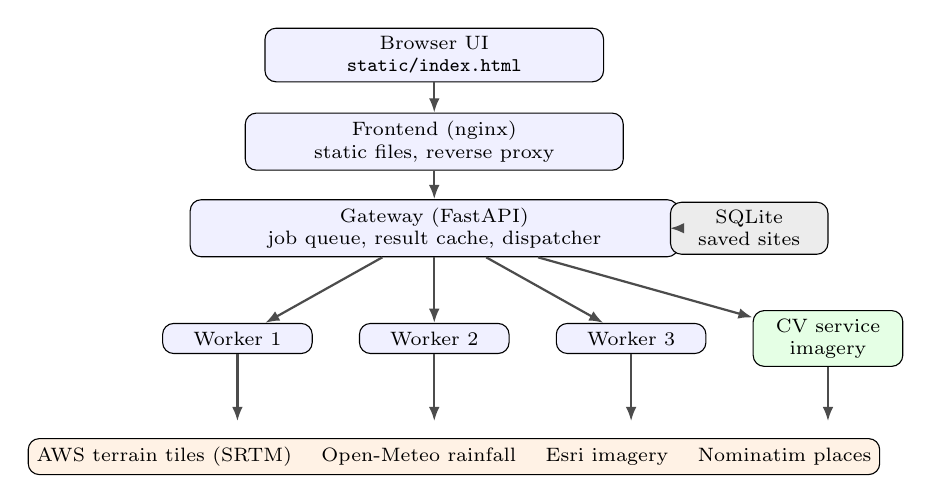
\begin{tikzpicture}[
    box/.style={draw, rounded corners, align=center, font=\scriptsize, fill=blue!6, inner sep=3pt},
    ext/.style={draw, rounded corners, align=center, font=\scriptsize, fill=orange!10, inner sep=3pt},
    db/.style={draw, rounded corners, align=center, font=\scriptsize, fill=gray!15, inner sep=3pt},
    cv/.style={draw, rounded corners, align=center, font=\scriptsize, fill=green!10, inner sep=3pt},
    arr/.style={-{Latex[length=1.8mm]}, thick, gray!60!black}
    ]
    \node[box, minimum width=4.3cm] (browser) at (3.9,7.4) {Browser UI\\\texttt{static/index.html}};
    \node[box, minimum width=4.8cm] (frontend) at (3.9,6.3) {Frontend (nginx)\\static files, reverse proxy};
    \node[box, minimum width=6.2cm] (gateway) at (3.9,5.2) {Gateway (FastAPI)\\job queue, result cache, dispatcher};
    \node[db, minimum width=2.0cm] (dbnode) at (7.9,5.2) {SQLite\\saved sites};
    \node[box, minimum width=1.9cm] (w1) at (1.4,3.8) {Worker 1};
    \node[box, minimum width=1.9cm] (w2) at (3.9,3.8) {Worker 2};
    \node[box, minimum width=1.9cm] (w3) at (6.4,3.8) {Worker 3};
    \node[cv, minimum width=1.9cm] (cvnode) at (8.9,3.8) {CV service\\imagery};
    \node[ext, minimum width=9.6cm, align=center] (extnode) at (4.15,2.3)
      {AWS terrain tiles (SRTM) \quad Open-Meteo rainfall \quad Esri imagery \quad Nominatim places};

    \draw[arr] (browser) -- (frontend);
    \draw[arr] (frontend) -- (gateway);
    \draw[arr] (gateway) -- (dbnode);
    \draw[arr] (gateway) -- (w1);
    \draw[arr] (gateway) -- (w2);
    \draw[arr] (gateway) -- (w3);
    \draw[arr] (gateway) -- (cvnode);
    \draw[arr] (w1) -- (1.4,2.75);
    \draw[arr] (w2) -- (3.9,2.75);
    \draw[arr] (w3) -- (6.4,2.75);
    \draw[arr] (cvnode) -- (8.9,2.75);
  \end{tikzpicture}
  \caption{High-level system architecture. One Docker image, three roles.}
  \label{fig:architecture}
  \Description{A layered diagram. A browser talks to an nginx frontend, which forwards
    requests to a gateway. The gateway dispatches analyses to three worker processes and
    a CV imagery service, and keeps a SQLite store of saved sites. The workers and the
    CV service each call out to four external data sources: AWS elevation tiles,
    Open-Meteo rainfall, Esri imagery and Nominatim place search.}
\end{figure}

\subsection{Technology Stack}
\textbf{Backend.} Python 3.12, FastAPI and Uvicorn, Pydantic for request and response
models, NumPy, SciPy and Pillow for all numerical and raster work, and httpx for
outbound calls.

\textbf{Frontend.} A single \texttt{static/index.html} file, about 3,200 lines, with no
build step and no CDN dependency. Every chart is hand-written SVG rather than a
charting library.

\textbf{Database.} SQLite for saved analyses, chosen because the assignment's own
containers have no spare memory for a database server and a single file needs none.

\textbf{External APIs.} AWS's terrarium elevation tiles (SRTM, about 30 m, free and
keyless), with OpenTopography as an opt-in alternative; Open-Meteo's ERA5 rainfall
archive; Esri World Imagery for satellite classification; OpenStreetMap's Nominatim for
village search.

\textbf{Deployment.} Docker and docker-compose for a six-container local stack, plus
shell scripts that deploy the same image across the four lab containers, with automatic
retry over the lab's ssh link.

The assignment brief suggests OpenCV and Leaflet as likely tools. Neither is used.
Installing OpenCV or GDAL on a 512 MB container with no root access was judged too
fragile to depend on for a live demo, and NumPy and SciPy already cover every image
operation the project needs, including thresholding, morphological opening, connected
components, and marching squares for contour generation. Leaflet was not adopted
either. A hand-rolled map already existed before the area-selection feature was added,
and porting it to a mapping library would have cost more time than adding a draw tool
to the existing one, while putting a CDN fetch on the critical path of a live demo.

%% =====================================================================
\section{Methodology}
\label{sec:methodology}

\subsection{Terrain and Elevation Analysis}
The analysis needs one thing from either input path: a grid of heights, called a
\texttt{DEM} in the code, with its resolution and its coordinate frame attached.
Everything downstream reads only that object.

From an uploaded contour sheet, every vertex of every contour line becomes a point with
a known height, found by trying four strategies in turn, 3D coordinates, an extended
data field, the placemark name, or the folder name, and keeping the first one that
explains at least 90\% of the file. The points are triangulated and interpolated onto a
square grid whose resolution is worked out from the contour spacing in the file, not
fixed in advance.

From a drawn map area, elevation comes from AWS's terrarium tiles. Each pixel decodes
to a height in metres from its red, green and blue channels. Tiles are chosen at a zoom
level whose ground resolution matches the contour path's own grid, mosaicked, and
resampled onto the same local grid the contour path uses, so the rest of the pipeline
cannot tell the two apart.

Both paths share the same cleanup steps. Interpolating or decoding whole-metre heights
produces a flat, stair-stepped surface, so a Gaussian smoothing pass, tuned to the input
resolution, turns it back into a slope. Any remaining depressions are removed by
priority-flood pit filling, so water always has somewhere to go. Contour lines can also
be generated back out of any DEM by marching squares, which satisfies the assignment's
contour-visualisation requirement for a drawn area with no uploaded sheet.

\subsection{Catchment Area Delineation}
Flow direction is computed with D8 steepest descent: each grid cell sends its water to
whichever of its eight neighbours has the steepest downhill slope, with diagonal
neighbours corrected for their longer distance. Because every cell's receiver is
strictly lower than the cell itself, sorting all cells by descending height gives a
valid processing order, and one pass down that order accumulates how much water passes
through every cell. A catchment is then delineated by walking this pointer structure
upstream from a chosen outlet, collecting every cell whose water eventually reaches it.

Candidate pond sites are found by three rules applied in order: the cell must sit on a
channel that drains at least a fixed share of the mapped area, the local slope must be
buildable, and the site must stand at least 3 m above the nearest channel that drains
more than 150 ha, so that the recommendation is never a section of the river itself.
Sites are ranked by catchment area, and each chosen site's entire upstream area is
removed before the next site is picked, so that alternative sites are independent
sub-basins rather than points strung along one stream.

Every catchment is cross-checked by recomputing it on three further grids at different
resolutions. Agreement across all four is reported as a confidence level and an
uncertainty band, rather than a single number that hides how much the answer depends on
grid resolution. A catchment whose boundary runs along the edge of the analysed area is
flagged, since its true extent may continue beyond what was measured.

\subsection{Rainfall Data Integration}
Ten years of daily rainfall are queried from Open-Meteo's ERA5 archive for the chosen
point and aggregated into an annual total, a rain-day count, and monthly means. If the
service cannot be reached, a documented regional climatology answers instead and the
response says so. Runoff is computed with the SCS curve number method applied to each
individual rain day and summed for the year, rather than to the year's total rainfall
as one storm. Applying it to a whole year at once returns a runoff coefficient over
90\%, which no real catchment produces; applied per rain day it returns 8\% to 16\% on
the terrain tested, which matches what is expected of rural Indian catchments.

%% =====================================================================
\section{Implementation}
\label{sec:implementation}

\subsection{Backend and API Design}
Table~\ref{tab:api} lists the main endpoints. All routes are versioned under
\texttt{/api/v1}, and the two analysis entry points, an uploaded sheet or a drawn area,
return exactly the same response shape, so the frontend renders either one the same
way. Every error, from any endpoint, comes back in one shape:
\texttt{\{status, code, detail, hint\}}, with a stable machine-readable code and a
human-readable hint. No authentication is required to call the API; see
Section~\ref{sec:csd-themes} for why.

\begin{table}[h]
  \caption{Main API endpoints}
  \label{tab:api}
  \begin{tabular}{p{3.6cm}p{3.6cm}}
    \toprule
    Method \& path & Purpose \\
    \midrule
    \texttt{POST /analyzeArea} & Analyse a drawn area (bbox or polygon) \\
    \texttt{POST /analyzeContour} & Analyse an uploaded contour sheet \\
    \texttt{POST/GET /jobs}, \texttt{/jobs/\{id\}} & Same analyses, asynchronously, with progress \\
    \texttt{POST /renderMap} & Either analysis, drawn as a PNG \\
    \texttt{POST /contours} & Contour lines, from a file or the DEM \\
    \texttt{POST /imagery/detectPonds}, \texttt{/land/available} & Existing water and available land from imagery \\
    \texttt{GET/POST /ponds} & Save, list and reopen analyses \\
    \texttt{GET /places}, \texttt{/rainfall} & Village search; ten years of rainfall for a point \\
    \texttt{GET /cluster}, \texttt{/health} & Cluster load; liveness and limits \\
    \bottomrule
  \end{tabular}
\end{table}

Errors from third-party services are handled, not just caught. A rainfall lookup that
fails falls back to a documented climatology. A failed basemap tile is retried after
five minutes rather than cached as permanently missing. A place-name search is retried
once before it is reported unavailable. A selection too large for the memory budget is
refused immediately with a named \texttt{422} rather than left to run out of memory,
and an overloaded cluster returns \texttt{503} with a retry hint instead of letting
requests queue until they time out.

\subsection{Frontend and Visualization}
The interface, shown in Figure~\ref{fig:ui}, is a single page. A user searches for a
village or draws a box or polygon directly on the map, with a live area readout checked
against the service's limits as they draw. Results appear as three headline figures,
pond location, catchment area, and expected water a year, alongside ranked alternative
sites with the reasons each was chosen. Layers can be toggled for the satellite,
street, or terrain basemap, contours, catchments, the flow network, and the existing
water and unavailable land read from imagery. A rainfall chart and a stage-storage
curve are drawn as hand-rolled SVG. Results can be saved, reopened, exported as GeoJSON
or a PNG map, or printed, through a single export menu.

\begin{figure}[h]
  \centering
  \includegraphics[width=0.88\linewidth]{docs/figures/phase3_area_result.jpg}
  \caption{The application interface: an area drawn on the map, analysed from free
    elevation tiles, with the recommended site, its catchment, the flow network, and
    generated contour lines overlaid.}
  \label{fig:ui}
  \Description{A screenshot of the web application. A dashed white rectangle marks the
    user's selection over satellite imagery. A blue polygon marks the recommended
    catchment with its outlet marker and flow path, two smaller alternative sites are
    marked nearby, and orange contour lines are drawn under everything. A right-hand
    panel lists the pond location, catchment area, and expected water per year.}
\end{figure}

\subsection{Database and Storage}
Saved analyses are persisted in a single SQLite file on the gateway's volume, looked up
by id and listed newest first. Three caches sit ahead of it in the request path: an
elevation-tile cache on each worker's own disk, keyed by tile source, zoom, and
coordinates; a rainfall cache at the gateway, keyed by rounded latitude and longitude;
and a full-result cache at the gateway, keyed by a hash of the request's bounding box
and parameters. A repeated query answers from the result cache in about 10 ms, against
roughly 2 s for a first, cold query.

%% =====================================================================
\section{CSD Themes and Topics Applied in the Project}
\label{sec:csd-themes}

Table~\ref{tab:csd-themes} maps core computer system design themes onto where each
appears in this project. Where a theme was deliberately not built out, the table gives
the reason rather than leaving it blank.

\begin{table*}[t]
  \caption{Mapping of core CSD themes/topics to their use in this project}
  \label{tab:csd-themes}
  \footnotesize
  \renewcommand{\arraystretch}{0.88}
  \setlength{\tabcolsep}{4pt}
  \begin{tabular}{p{2.6cm}p{4.9cm}p{6.1cm}}
    \toprule
    CSD Theme/Topic & Where used in the project & Justification / design rationale \\
    \midrule
    API Design (REST) & \texttt{/api/v1/analyzeArea}, \texttt{/api/v1/analyzeContour}, both under \texttt{/v1} & One response schema for both entry paths and one error envelope (\texttt{status}, \texttt{code}, \texttt{detail}, \texttt{hint}), so a client handles either the same way. \\
    Load Balancing & The gateway's least-busy dispatcher, compared against the lab's existing round-robin Go balancer & Each worker holds one analysis at a time on 512 MB, so dispatch choice changes tail latency directly; least-busy measured 9\% to 12\% lower p95/p99 at equal throughput. \\
    Caching & Tile cache per worker, rainfall cache by coordinate, result cache by request hash & Tiles are immutable, rainfall APIs are rate-limited from a shared IP, and a repeated query returns in 10 ms instead of 2 s. \\
    Database Indexing / Query Optimization & SQLite primary-key lookup for saved analyses (\texttt{app/store.py}) & The store is small at this scale, so the primary key already covers both queries the API needs. An \texttt{rtree} spatial index is the natural next step if saved sites grew into the thousands. \\
    Concurrency / Asynchronous Processing & Async job API (\texttt{POST /jobs}, \texttt{GET /jobs/\{id\}}) on a worker thread pool & Keeps \texttt{/health} responsive during a multi-second analysis and lets the page show real per-stage progress instead of blocking. \\
    Microservices vs. Monolith & One image, one codebase; role (gateway, worker, or CV service) set by an environment variable at start & Four containers share no filesystem and this was built solo; one image deployed everywhere avoids keeping several codebases in sync for no functional gain. \\
    Design Patterns & Strategy: one \texttt{ElevationProvider} interface behind a terrarium-tile and an OpenTopography implementation, the same shape for rainfall & Adding a data source touches only its provider. The rest of the pipeline depends only on the \texttt{DEM} object it produces, which is also why the upload path and the map-drawing path share all downstream code. \\
    Authentication / Authorization & Not implemented & No private data or per-user state exists yet, and a saved analysis is not tied to an identity. An API key on the \texttt{/ponds} write endpoints is the natural next step if that changed. \\
    Containerization / Deployment & A \texttt{Dockerfile}, a six-service \texttt{docker-compose} stack, and scripts that deploy the same image to the four lab containers with retry over a flaky link & One command reproduces the whole system for grading, and every container is capped at 512 MB to match the assignment's own limit. \\
    Error Handling and Resilience & Structured \texttt{\{status, code, detail, hint\}} errors; a rainfall climatology, a hillshade basemap, and a named \texttt{422} or \texttt{503} in place of a crash or a hang & A field tool should degrade, not fail, when one of several third-party services is briefly unavailable. \\
    Algorithms and Complexity & D8 flow routing and priority-flood pit filling, both near-linear via one sort and one pass; marching squares for contour generation & The grid can hold hundreds of thousands of cells and the 512 MB container leaves no room for anything worse than near-linear. \\
    Testing Strategy & 588 automated tests, including an analytically solvable case with a provable answer and a two-path cross-check against the surveyed sheet & Passing tests confirm the code runs; the analytic and mass-balance checks are what confirm the catchment area it reports is actually correct. \\
    Version Control / CI-CD & Git, one logical change per commit. No automated pipeline & The four deployment targets are fixed, memory-capped containers with no spare runner capacity; running the full test suite locally before each commit substituted for CI at this project's scale. \\
    \bottomrule
  \end{tabular}
\end{table*}

Three of these decisions mattered more than the rest to how the system behaves under
the assignment's own constraints. Load balancing and dispatch decided how much of the
memory limit could actually be used: with each worker holding only one analysis at a
time, an idle worker sitting behind a busy one is wasted capacity, and moving from
round-robin to a queue-aware dispatcher is what Section~\ref{sec:results} measures.
Caching decided whether the system felt instant or slow, since the same elevation
tiles and rainfall records are requested again and again with no reason to fetch or
recompute them twice. The choice of one image with a role, rather than a full
microservice split, was a deliberate trade against the brief's own suggestion. It was
made because the four systems share no storage and this was built by one person on a
deadline; splitting further would have added coordination cost without adding any
capability the assignment asks for.

%% =====================================================================
\section{Results and Evaluation}
\label{sec:results}

\subsection{An Example Site}
Figure~\ref{fig:results} shows the system analysing the sample area supplied with the
assignment, an 852 ha rectangle near the Shivnath river (81.28 to 81.31 E, 21.24 to
21.26 N). The recommended site sits at 21.2437 N, 81.2861 E, with a catchment of 87 ha
(uncertainty $\pm$10.8 ha, cross-grid confidence medium). At the site's ten-year mean
rainfall of 1,397 mm a year, the catchment delivers about 96,500 m\textsuperscript{3} of
runoff annually, enough to fill a 3 m deep, 586 m\textsuperscript{3} pond roughly 165
times over in a year. Two alternative sites are shown as well, each an independent
sub-basin rather than a second point on the same stream as the first.

\begin{figure}[h]
  \centering
  \includegraphics[width=0.88\linewidth]{docs/figures/phase3_water.jpg}
  \caption{Rainfall and runoff for the recommended site: monthly means with the monsoon
    highlighted, and the ten-year annual series against its mean.}
  \label{fig:results}
  \Description{A screenshot of the application's water panel, showing a bar chart of
    mean monthly rainfall with June to September highlighted, a second bar chart of
    ten years of annual rainfall totals against a dashed mean line, and a table of
    curve number, retention, initial abstraction, runoff depth and coefficient, and
    annual runoff volume for the recommended site.}
\end{figure}

\subsection{Accuracy Against a Surveyed Sheet}
To check the free-data path against a source of truth, the same rectangle was analysed
twice: once from the provided 1 m contour survey, and once from the free 30 m SRTM
tiles, drawn as an area exactly as a user would draw it. Table~\ref{tab:validation}
summarises the result.

\begin{table}[h]
  \caption{The surveyed sheet against the free-data map path, same ground}
  \label{tab:validation}
  \begin{tabular}{p{2.6cm}p{2.1cm}p{2.5cm}}
    \toprule
    Metric & 1 m survey & 30 m map path \\
    \midrule
    Elevation range & 267--298 m & 266--298 m \\
    DEM agreement & --- & RMSE 0.26 m \\
    Recommended site & 21.2439 N, 81.2900 E & 21.2437 N, 81.2861 E \\
    Site offset & \multicolumn{2}{c}{402 m, same valley} \\
    Catchment area & 66.3 ha & 87.0 ha (+31\%) \\
    Catchment overlap & \multicolumn{2}{c}{IoU 0.53} \\
    Annual runoff & 127{,}040 m\textsuperscript{3} & 166{,}610 m\textsuperscript{3} \\
    Grid size & 638{,}472 cells & 60{,}606 cells \\
    Runtime & 10.0 s & 0.49 s \\
    \bottomrule
  \end{tabular}
\end{table}

The two elevation models agree to 0.26 m, closer than SRTM's typical accuracy against a
field survey, which suggests the provided sheet was itself drawn from SRTM-class data.
This mainly validates the software path: tile decoding, the margin analysed around a
drawn selection, and routing on a coarser grid, rather than SRTM against an independent
physical benchmark. Where the two paths disagree, the 17.8 m grid against the survey's
3.1 m is the reason: a coarser grid moves where two channels meet by a cell or two,
which is enough to redraw which ground drains where. Catchment area and its uncertainty
should be read at the map path's own resolution, and a construction-grade pond depth
still needs a proper survey.

\subsection{Performance}
Table~\ref{tab:scaling} was measured against a docker-compose deployment with every
container capped at 512 MB, the same limit as the four lab systems provided for this
assignment. As of this report, the multi-worker deployment described in
Section~\ref{sec:architecture} had not yet been run on the actual lab hosts; the
earlier, single-container service from the assignment's first phase is what is
currently live there. The figures below are reported as the closest available
measurement under an identical memory envelope, and Section~\ref{sec:discussion} states
this as an open item.

\begin{table}[h]
  \caption{Throughput and latency against worker count}
  \label{tab:scaling}
  \begin{tabular}{ccccc}
    \toprule
    Workers & Throughput & p50 & p95 & Peak memory \\
    \midrule
    1 & 1.34 req/s & 4.11 s & 7.65 s & 204 MiB \\
    2 & 2.10 req/s & 2.60 s & 4.50 s & 220 MiB \\
    3 & 3.54 req/s & 1.17 s & 2.99 s & 224 MiB \\
    \bottomrule
  \end{tabular}
\end{table}

Three workers give 2.6 times the throughput of one. A selection over
100 km\textsuperscript{2} is refused with a named \texttt{422} in about 25 ms rather
than attempted. Under a burst of 24 large selections against a queue capped at 4, the
system answered 7 and returned \texttt{503 busy} for the other 17, instead of letting
all 24 time out. Peak worker memory across the whole test matrix was 276 MiB of the
512 MiB available.

%% =====================================================================
\section{Discussion and Limitations}
\label{sec:discussion}

The map path trades accuracy for speed and reach. Its 17.8 m grid reports a catchment
31\% larger than the same site measured from a 1 m survey, with 0.53 catchment overlap
between the two. This is resolution, not an error in the algorithm, since the same code
runs both paths and the mass-balance and analytic-answer tests hold on both.

Pond capacity is the part most affected by data resolution. Whole-metre SRTM heights
put small ridges around every hollow, so the map path's stage-storage curve spills
early: the example site holds 586 m\textsuperscript{3} where a comparable surveyed site
holds about 21,000 m\textsuperscript{3}. Catchment area and runoff volume are reliable
enough to choose a site; the pond's final depth and capacity should still be designed
from a survey.

The imagery layer that flags existing ponds and unavailable land is a rule-based
screening step built from colour and texture thresholds in NumPy and SciPy, not a
trained model. It can read a flooded paddy field as open water, and it does not
separate tree cover from crops at the imagery's resolution. Every response that uses it
says so.

SRTM's own accuracy against real ground is not independently measured in this project,
because the only ground truth available, the provided survey, agrees with SRTM closely
enough that it was likely derived from similar data itself.

As noted in Section~\ref{sec:results}, the full four-container deployment and its
scaling measurement had not been run on the assignment's actual lab hosts at the time
of writing, only on an equivalent local stack under the same memory cap. No
authentication and no automated CI pipeline are implemented, for the reasons given in
Section~\ref{sec:csd-themes}.

%% =====================================================================
\section{AI Tool Usage Declaration}
\label{sec:ai-usage}

Claude (Anthropic, Sonnet 5) was used for one task on this project: turning the
assignment's report template into this filled-in report, drawing only on documentation
the author had already written while building and testing the system, the project
README and the technical notes in its \texttt{docs/} folder, the project's git history,
and screenshots generated by the running application. It also assembled the
architecture diagram in Figure~\ref{fig:architecture} and helped phrase and compress
the prose. It was not used to design the catchment algorithm, write the application
code, or decide the engineering trade-offs discussed in Section~\ref{sec:csd-themes};
those were made by the author over the course of the project and are documented, with
their supporting evidence, in the repository. Every claim, number and table in this
report was checked against the underlying documentation and code before submission.

%% =====================================================================
\appendix

\section{Source Code and Repository}
The complete source code, tests and documentation for this project are at:
\url{https://github.com/Akshats-git/Pond-Catchment-Analysis}

The system is deployed and live at \url{http://10.1.75.53:5229/}, and a video
walkthrough of the working, algorithm and demo is at \url{https://youtu.be/r1ir7I915W4}.

The repository is organised as follows.
\texttt{app/core/}: the terrain and hydrology analysis (DEM, flow routing, catchment
delineation, pond siting, runoff and storage, contour generation, GeoJSON export).
\texttt{app/providers/}: elevation and rainfall sources, each cached.
\texttt{app/cv/}: satellite imagery classification.
\texttt{app/routers/}, \texttt{app/schemas/}: the HTTP layer.
\texttt{app/jobs.py}, \texttt{app/store.py}: the job queue and saved-analysis
persistence.
\texttt{static/}: the frontend, one HTML file, no build step.
\texttt{deploy/}: deployment scripts for docker-compose and the lab containers.
\texttt{tools/}, \texttt{tests/}, \texttt{docs/}: the load generator, the automated
test suite, and the technical documentation this report draws on.

\end{document}
\endinput
